\section{Software Architektur}
\label{sec:software-architektur}

Die Software-Architektur des Projektes definiert die Möglichkeiten bei der Implementierung, die man zum Erfüllen der Anforderungen zur Verfügung hat. Deshalb war es wichtig, sich ausreichend Gedanken zu machen, um später im Projekt dann nicht feststellen zu müssen, dass die gewählte Architektur für die Anforderungen ungeeignet ist. Die Hauptanforderung an die Architektur ist selbstverständlich die Bereitstellung eines Kommunikationskanals zwischen Controllern und Robotern. Es muss möglich sein Richtungs- und Geschwindigkeitsänderungen seitens der Anwender an die Roboter mitzuteilen. Der Status des Roboters soll jederzeit ausgewertet und entsprechend darauf reagiert werden können. Hierzu gehören das automatische Anfahren der Ladestation bei geringem Akkustand und die Übertragung der Bilddaten. Außerdem sollen Zustandsänderungen des Spiels, die nicht vom Roboter oder Controller direkt ausgehen erkannt und korrekt verarbeitet werden. 

Ausgehend von diesen Bedingungen, die die Architektur erfüllen muss, kamen folgende Architekturen in Frage:

Eine \textbf{Client-Server-Architektur} bei der ein Server zentral die Kommunikation verwaltet. Hierbei findet keine Kommunikation zwischen den Steuergeräten und den Robotern direkt statt. Die Torerkennung kommuniziert direkt mit dem Server, ohne dass Roboter und Controller zwangsweise etwas davon mitbekommen. Sowohl die Roboter, als auch die Controller nehmen die Rolle eines Clients ein. Dadurch ist es Möglich, dass eine Steuerung des Servers stattfinden kann, ohne dass ein Controller verbunden ist. Zusätzlich ist es in dieser Architektur möglich beliebig viele Clients anzubinden. Durch die Trennung von Client und Logik können die Controller beliebig erweitert und ausgetauscht werden, ohne die eigentliche Spiellogik zu ändern.

\begin{figure}
	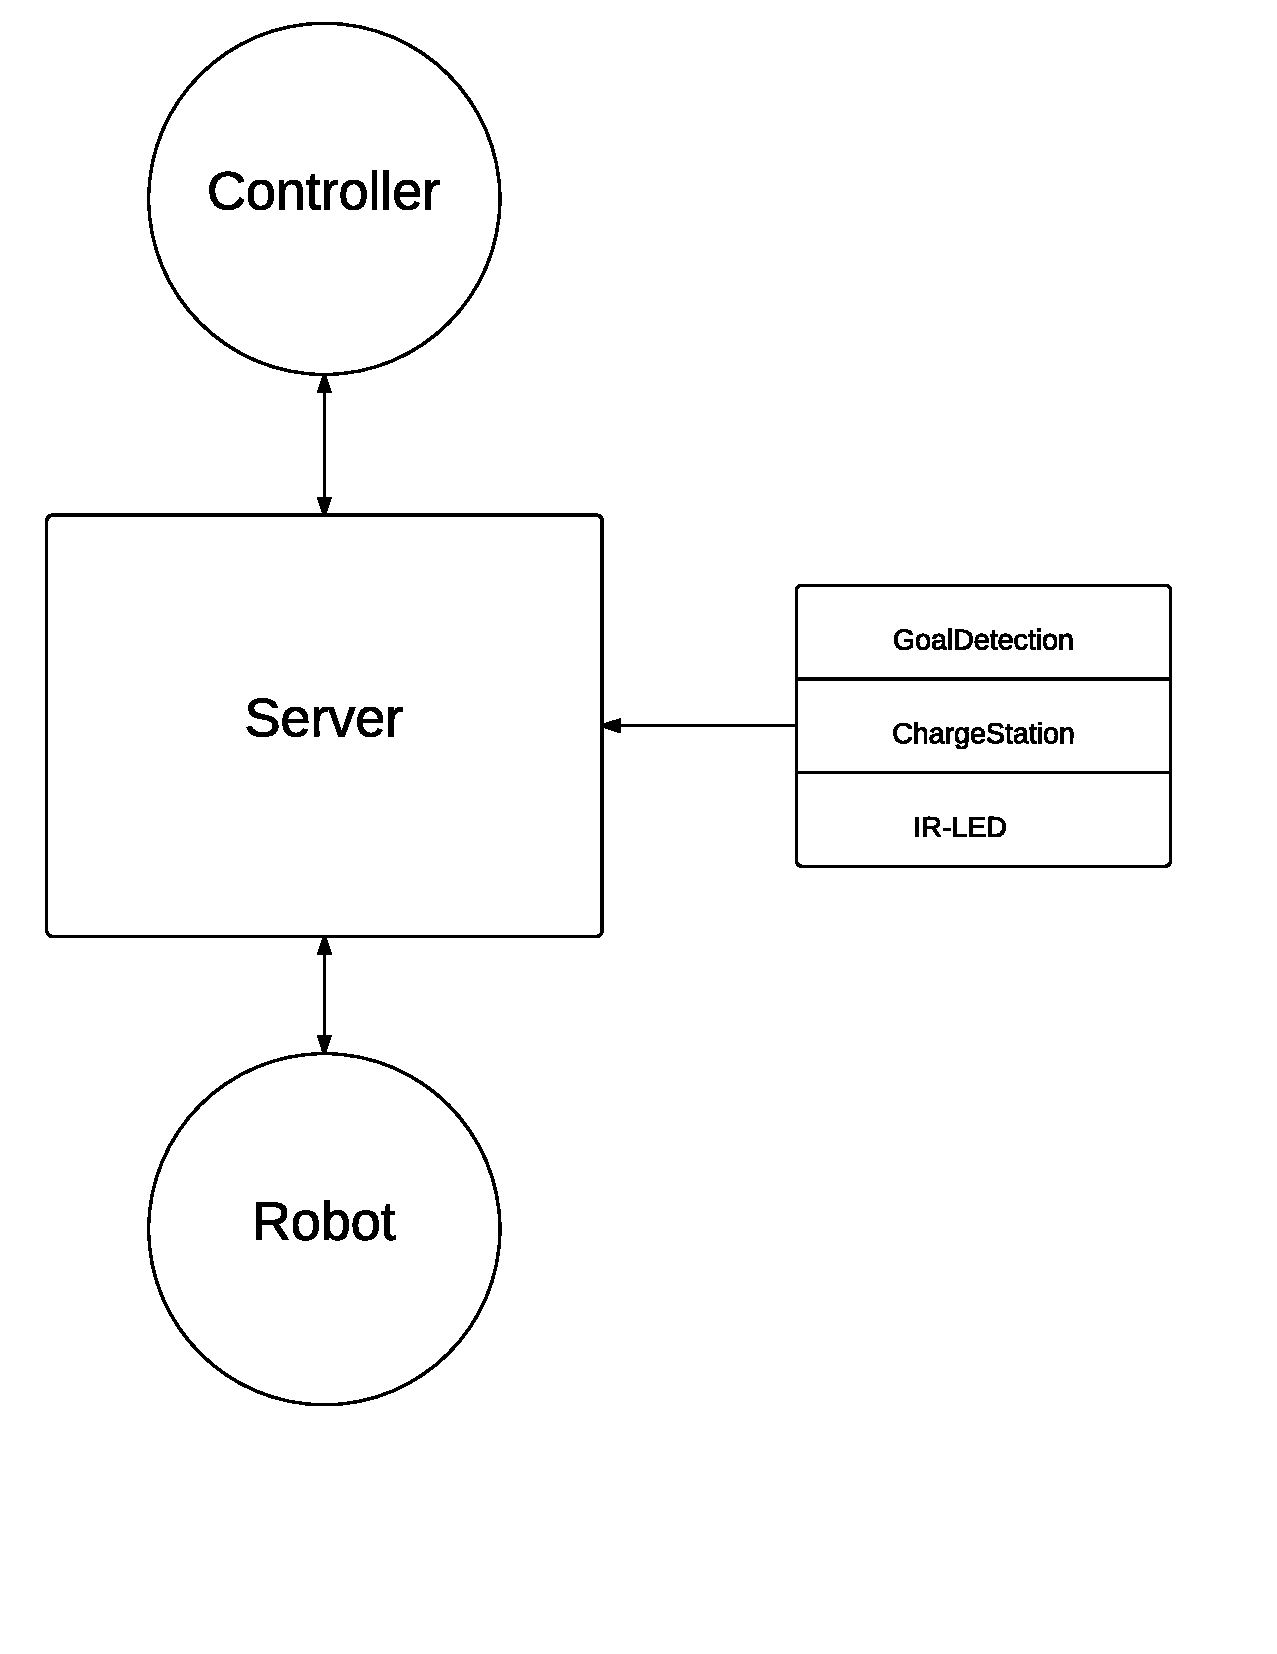
\includegraphics[height=0.5\textheight]{images/client-server_architektur.pdf}
	\caption{Client-Server Architektur}
	\label{fig:client-server_architektur}
\end{figure}


Eine Architektur, die Roboter und Controller \textbf{paarweise} verbindet. Bei dieser Architektur wird jedem Roboter ein Controller zugewiesen, der genau diesen steuert. Die peripheren Geräte senden direkt an die Controller. Auch die gesamte Spiellogik ist in den Controller gekapselt. Ein Vorteil dieser Architektur ist die geringe Latenz bei der Befehlsübermittlung. Im Vergleich zur Client-Server-Architektur gibt es hier keinen dritten Knoten, über den die Übertragung abgehalten wird, wodurch sich die benötigte Zeit halbiert.

\begin{figure}
	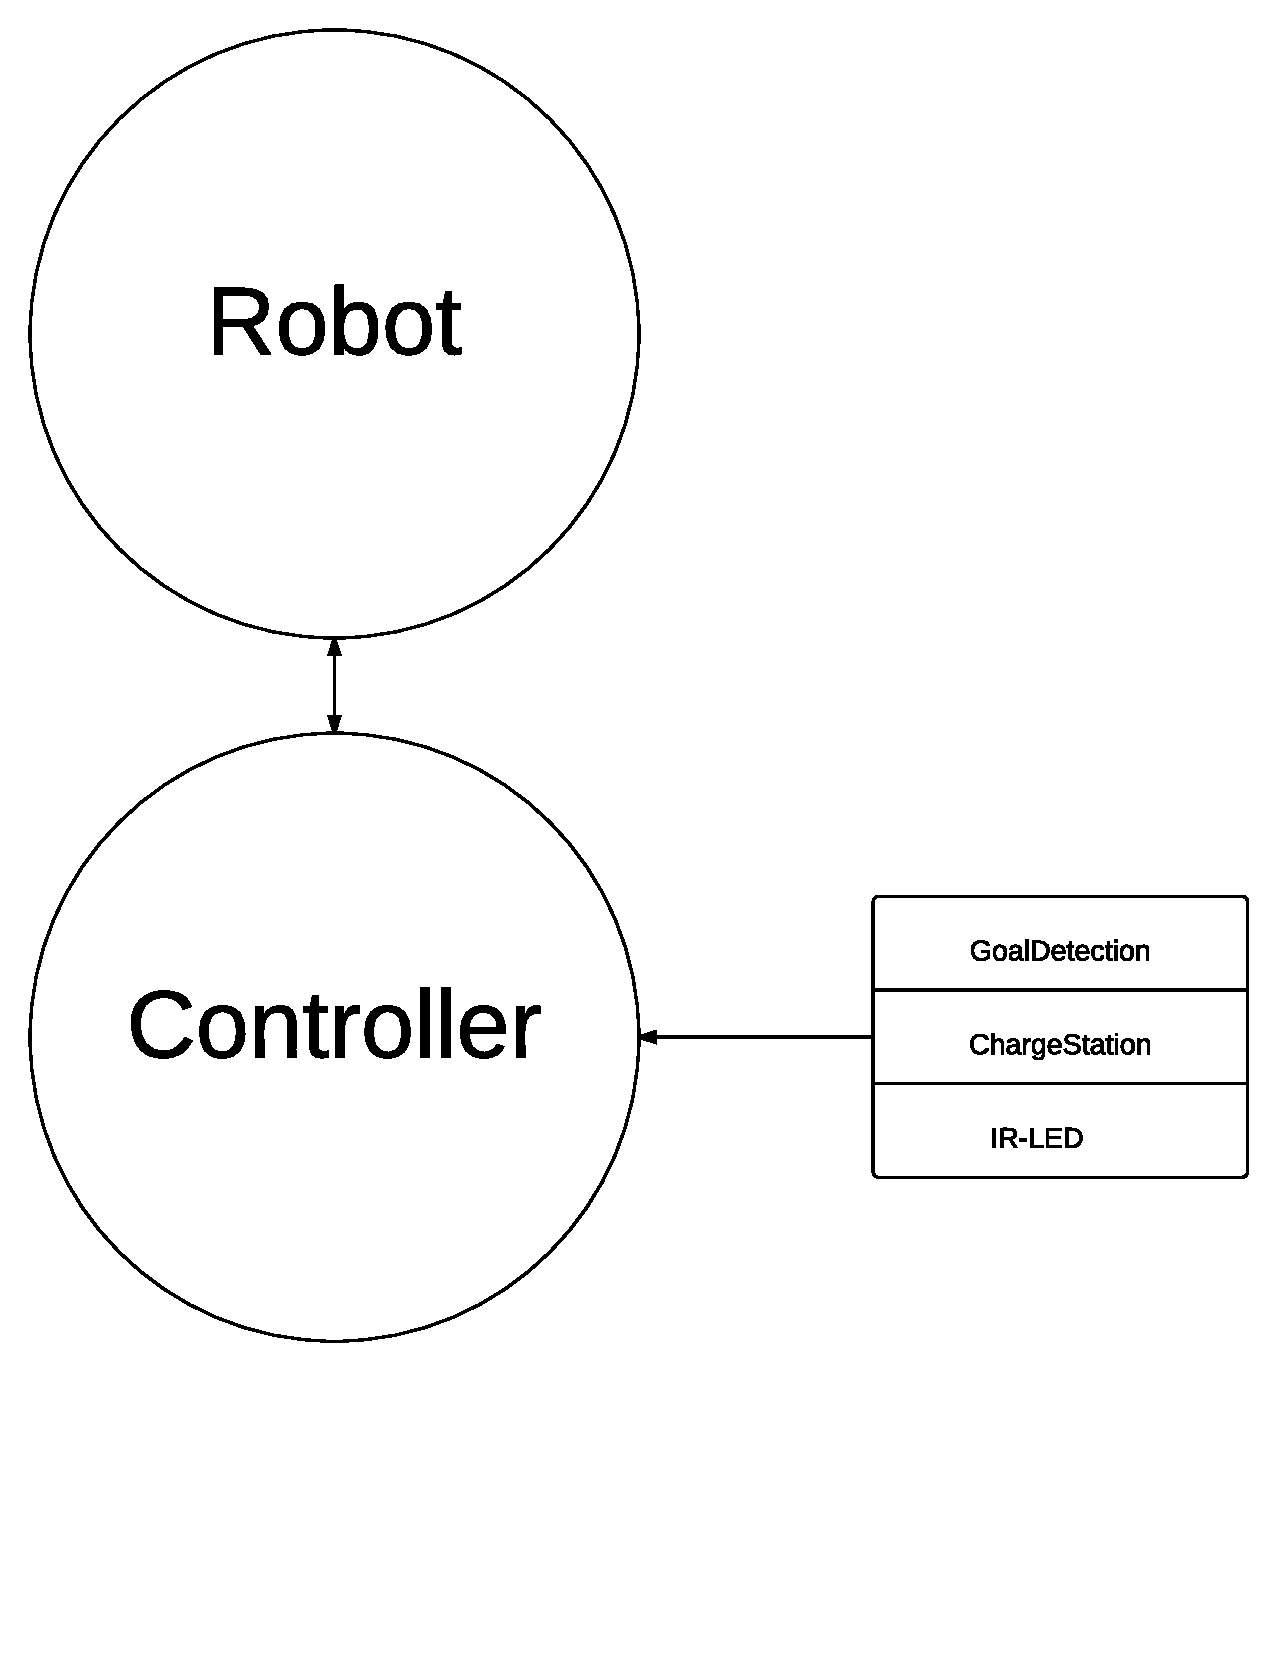
\includegraphics[height=0.5\textheight]{images/paarweise_architektur.pdf}
	\caption{Paarweise Architektur}
	\label{fig:paarweise_architektur}
\end{figure}


Nach Abwägung der Vor- und Nachteile beider Architekturen schien es vernünftiger sich für die Client-Server-Architektur zu entscheiden. Einer der Hauptgründe hierfür ist die hervorragende Erweiterbarkeit in Bezug auf die Controller. Da keine Logik in den Controllern ist, muss sie auch nicht für jeden Controller separat entwickelt werden, beziehungsweise nicht einmal vorhanden sein. Gerade für das Auffinden der Ladestation wäre es nicht sinnvoll, solange mit dem Laden zu warten, bis ein Controller verbunden ist, nur um dann festzustellen dass der Akku leer ist und der Roboter erst geladen werden muss, bevor gespielt werden kann. Auch in Anbetracht der Informationskapselung, die bei der paarweisen Architektur entstehen würde, ist es sinnvoller die Client-Server-Architektur zu bevorzugen. Nur wenn alle Informationen über das Spiel, also über jeden Roboter und jeden Controller zentral verwaltet werden, ist es möglich die Informationen korrekt zu verarbeiten und entsprechend darauf zu reagieren. So wird zum Beispiel ein neues Spiel gestartet, sobald beide Roboter mit einem Controller verbunden sind. Bei der paarweisen Architektur wäre dies nicht möglich, da die beiden Controller-Roboter-Einheiten vom jeweils anderen keine Informationen über deren Status erhalten.